\documentclass[12pt, english, letterpaper]{kuthesis}
\usepackage{mathptmx}
\renewcommand{\sfdefault}{lmss}
\renewcommand{\ttdefault}{lmtt}
\usepackage[T1]{fontenc}
\usepackage[utf8]{inputenc}
\usepackage{geometry}
\geometry{verbose,tmargin=1in,bmargin=1in,lmargin=1in,rmargin=1in}
\setcounter{secnumdepth}{3}
\setcounter{tocdepth}{3}
\usepackage{color}
\usepackage{babel}
\usepackage{url}
\usepackage{graphicx}
\usepackage{setspace}
\usepackage{esint}
\usepackage[authoryear]{natbib}
\doublespacing
\usepackage[unicode=true,
 bookmarks=true,bookmarksnumbered=false,bookmarksopen=false,
 breaklinks=true,pdfborder={0 0 0},pdfborderstyle={},backref=false,colorlinks=true]
 {hyperref}
\hypersetup{pdftitle={Promise Land},
 pdfauthor={Andrei Elliott},
 pdfsubject={Javascript-style Promises with Strong Typing},
 urlcolor={black},citecolor={black},allcolors={black}}

\usepackage{listings}
\usepackage{fancyvrb}
\usepackage{hyperref}
\usepackage[nameinlink, noabbrev]{cleveref}
\usepackage{tikz}

\usetikzlibrary{calc, matrix, positioning}
\tikzset{ gap/.style = {preaction={draw, line width=2pt, white}} }


\newcommand{\lit}[1]{\texttt{#1}}

\DefineVerbatimEnvironment{code}{Verbatim}{}
%\newenvironment{code}{\Verbatim}{\endVerbatim}

\title{Promise Land\\
\large Proving Correctness with Strongly Typed Javascript-Style Promises}
\author{Andrei Elliott}

\priorcreds{}

\dept{Electrical Engineering and Computer Science}
\degreetitle{Master of Science}
\papertype{Project Report}

\committee {Matt Moore}	{Perry Alexander}	{Drew Davidson}	{}	{}	{}	{}
\role      {Chair}	{}	{}	{}	{}	{}	{}



\makeatletter
\@printd@testrue
\datedefended{Friday May 6, 2022}
\dateapproved{-}
\makeatother

\begin{document}

\begin{romanpages}
  \maketitle
  \begin{abstract}
    Code that can run asynchronously is important in a wide variety of situations, from user interfaces to communication over networks, to the use of concurrency for performance gains.  One widely-used method of specifying asynchronous control flow is the \lit{Promise} model as used in Javascript.  \lit{Promise}s are powerful, but can be confusing and hard-to-debug.  This problem is exacerbated by Javascript’s permissive type system, where erroneous code is likely to fail silently, with values being implicitly coerced into unexpected types at runtime.

The present work implements Javascript-style \lit{Promise}s in Haskell, translating the model to a strongly typed framework where we can use the type system to rule out some classes of bugs.
Common errors – such as failure to call one of the callbacks of an executor, which would, in Javascript, leave the \lit{Promise} in an eternally-\emph{pending} deadlock state – can be detected for free by the type system at compile time and corrected without even needing to run the code.

We also demonstrate that \lit{Promise}s form a monad, providing a monad instance that allows code using \lit{Promise}s to be written using Haskell’s \emph{do notation}.
  \end{abstract}
%  \tableofcontents {}
\end{romanpages}

\chapter*{Introduction}
One widely used model of concurrency is Javascript's Promises.  A promise works in some ways like a lazy value, in that it will at some point contain the result of a computation, but does not stop flow of control in the current thread to compute that value.  Unlike a value with lazy semantics, a promise can immediately begin computation in a separate thread as opposed to waiting for the result to be requested by some other computation.

Promises are composable: using \lit{then} and \lit{catch}, we can chain a promise onto the end of a different one creating a new promise that continues computation after the first has succeeded or failed respectively.  Additionally, \lit{Promise}s can be combined in parallel, with a variety of distinct semantics such as waiting for the first success or for the first completion irrespective of success or failure.

\cite{madsen} note that programmers often make mistakes when writing code involving promises and there are no static checks to detect them.

We build a model of \lit{Promise}s in Haskell and discuss what we gain by using a stronger type system.  In particular, we show that some classes of errors can be caught automatically by the type checker.
\chapter*{Motivation}
\lit{Promises} as adopted by Javascript use model initially proposed in \cite{friedman}.
[Discussion of the adoption of the promises model in Javascript; will have to see what I can find citations for.]

Promise objects are a good candidate for parameterized types: they yield a value upon success or failure, and it would be nice to be able to check statically that these values and the functions that they will be passed to all agree on the types involved.

The operation \lit{then} should ``chain promises together'' by accepting a function that converts a regular value to a promise, then applying it to a promise with that return type by waiting for it to finish before calling the function.  Note that this operation is very similar to \lit{>>=} [give type signature here?], suggesting that promises can be thought of as monads.  (We also note that it is trivial to wrap an arbitrary value into a promise so \lit{return} poses no problem.  In practice, we define a separate constructor for this case to avoid forking off an entire new thread to do no computation and hand back the same result immediately.)

\chapter*{Background}
\section*{Haskell}
[HS type signature syntax - mention here that I'm using \lit ? in type signatures I'm discussing as a metavariable, not real syntax?]
[IO monad, do notation]
[forkIO, description of MVar]
[maybe discuss GADTs briefly ?]

\section*{Promises}
[Promises here $\neq$ lazy values, despite terminology clash w/ e.g. Scheme]
\lit{Promise}s can be in one of three states.  The \emph{pending} state represents a \lit{Promise} that is still running.  A \lit{Promise} that has completed with a success value is in the \emph{fulfilled} state; the process of moving from \emph{pending} to \emph{fulfilled} is referred to as the \lit{Promise} \emph{resolving}.  The state for a failed \lit{Promise} is called \emph{rejected} and to \emph{reject} a \lit{Promise} is to move it from the \emph{pending} state to the \emph{rejected} state.  For a \lit{Promise} to \emph{settle}, it moves from \emph{pending} to either \emph{fulfilled} or \emph{rejected}.  \Cref{fig:states} summarizes this terminology.

\begin{figure}
\caption{states and transitions}
\label{fig:states}
\begin{center} 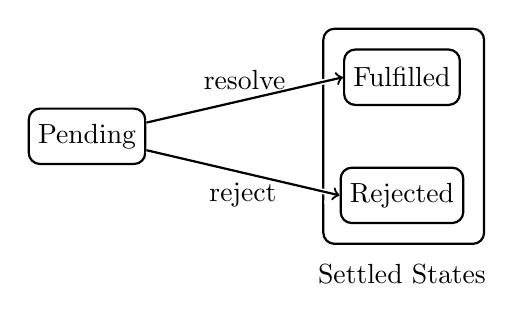
\begin{tikzpicture}
  \path (0,0) node[draw, thick, rounded corners, minimum height=2em, minimum width=4em] (pend) {Pending}
      ++(4,0.75) node[draw, thick, rounded corners, minimum height=2em, minimum width=4em] (ful) {Fulfilled}
      ++(0,-1.5) node[draw, thick, rounded corners, minimum height=2em, minimum width=4em] (rej) {Rejected}
      ++(0,-1) node {Settled States};

  \draw[rounded corners, thick] ($(ful.north west)+(-0.25,0.25)$) rectangle ($(rej.south east)+(0.25,-0.25)$);
  \draw[thick] (pend) edge[gap,->] node[above] {resolve} (ful.west) (pend) edge[gap,->] node[below] {reject} (rej.west);
\end{tikzpicture} \end{center}
\end{figure}

\section*{Comparison with Existing Concurrency Frameworks}
[Compare to push-pull frp]
[locks]


\chapter*{Haskell Implementation}

\section*{Making a Promise}
Javascript's \lit{Promise()} constructor builds a new promise object from an `executor' function.  The executor accecpts two callback functions the standard names resolutionFunc and rejectionFunc, one to call in the case of successful resolution and the other for failure.  The executor will, on a success/failure, call \lit{resolutionFunc}/\lit{rejectionFunc}, repectively, passing in the value of or reason for the success or failure.  Let's assume we want a promise with type \lit{Promise f p}, i.e. one where success results in a value of type \lit p and failure gives a reason with type \lit f.  To build one, \lit{resolutionFunc} will need to accept a value of type \lit p.  Since calling \lit{resolutionFunc} will settle the promise and therefore have effects elsewhere in the promise chain, its return type will have to be something wrapped in \lit{IO}, so we know \lit{resolutionFunc :: p -> IO ?}.  Similarly, \lit{rejectionFunc} must accept a \lit f, and calling it will also settle the promise, so \lit{rejectionFunc :: f -> IO ?}.  The executor function should accept \lit{resolutionFunc} and \lit{rejectionFunc} as parameters and is expected to end by calling exactly one of them, so we will expect it to have a proper tail call to one of the parameters.  This means its return type matches that of \lit{resolutionFunc} and \lit{rejectionFunc}, i.e. \lit{executor :: (p -> IO ?) -> (p -> IO ?) -> IO ?} and the \lit ?s for the two callbacks should be the same type.  For now, let's use \lit{()} as \lit ?, so that the callbacks have a return type of \lit{IO ()}, the conventional Haskell type for \lit{IO} actions that only have an effect (here, setting the Promise from \lit{Pending} state to one of the settled states) instead of containing a useful value.  Our function for building a \lit{Promise} object needs to accept a function with the type of \lit{executor} and give back a \lit{Promise} value, which must be contained in \lit{IO} because it has the side effect of running the \lit{executor} in another thread.  It thus has the type \lit{newPromise :: ((p -> IO ()) -> (f -> IO ()) -> IO ()) -> IO (Promise f p)}.  We can represent a \lit{Promise f p} by an \lit{MVar (Either f p)}.  Once the computation for the \lit{Promise} is complete, it can be written to with an \lit{Either f p} value, i.e. \lit{Left reason} for a failure or \lit{Right result} in the case of success.  \lit{newPromise} will also need to fork a thread that will run the executor and set up communication so that the final \lit{Promise} object will be updated with the results once they are available.  In total, we need to: create an \lit{MVar} which we'll call \lit{state}, then fork a thread that calls the executor, passing it callback functions that write the results to \lit{state}, and finally, return \lit{state} as a \lit{Promise} value.
\begin{code}
newPromise :: ((p -> IO ()) -> (f -> IO ()) -> IO ()) -> IO (Promise f p)
newPromise k = do
  state <- newEmptyMVar
  forkIO $ k (putMVar state . Right) (putMVar state . Left)
  return (Pending state)
\end{code}
% $
Since the constructor here is used to create \lit{Promise}s that are in the \emph{pending} state, we'll call it \lit{Pending}.  We could, in principle, use this same constructor to build \lit{Promise} values that we know have already succeeded or failed.  To get a promise that always succeeds with a value of \lit s, say, simply call \lit{newPromise} with an executor that immediately calls \lit{successFunc}, like so:
\begin{code}
newPromise (\ succeed fail -> succeed s)
\end{code}
This is inefficient, though, because it spawns an entire new thread in order to do absolutely nothing with it.  Instead, it is easy enough to define a constructor that marks a value as known to be the result of a sucessful computation (and a parallel one declaring a value to be the known reason for a failed computation).  These correspond to the promise being in the state \emph{fulfilled} or \emph{rejected}, repectively, so we will uses those terms as the names the constructors.  At this point, the \lit{Promise} type has the following form, in GADT syntax:
\begin{code}
data Promise :: * -> * -> * where
  Pending :: MVar (Either f p) -> Promise f p
  Fulfilled :: p -> Promise f p
  Rejected :: f -> Promise f p
\end{code}
What happens if we use a type other than \lit{()} in place of \lit ? in the \lit{newPromise} function?  Say we use the type $\tau$.  The executor function passed in must evaluate to an \lit{IO $\tau$}.  If the executor ends in a call to either \lit{resolutionFunc} or \lit{rejectionFunc}, it will work exactly the same no matter what type $\tau$ represents.  When using \lit{newPromise}, we can use the same code we did before in the \lit{$\tau = $()} case.  [When \lit{ executor} doesn't contain a tail-call to one of its argument functions, the type $\tau$ matters for whether \lit{newPromise executor} typechecks; in particular, it will be accepted if and only if whatever \lit{executor} is doing \emph{other than} calling one of its callbacks yields the result type \lit{IO $\tau$}. In this situation, the resulting \lit{Promise} will never settle and any further actions chained to it will never run.  Unintentionally causing this state of affairs in that manner is a [common (?check this)] cause of errors in javascript code using \lit{Promise}s. [cite]  If we were to select a type $\tau$ that doesn't appear as the result of normal code, we could have Haskell's type system automatically detect this entire class of bugs at compile time.  One option would be Haskell's \lit{Void} type, which has no constructors.  But there may be cases where we legitimately need a \lit{Promise} that will never resolve (for example, the Javascript standard specifes that the result of calling \lit{Promise.race()} on the empty list results in such a \lit{Promise}).  Furthermore, we need to create a value of type \lit{IO $\tau$} when implementing \lit{newPromise}.  Therefore, instead of using \lit{Void}, we create a new type unused anywhere else.  [could use \lit{Void} as \lit ? instead of \lit{()} - this would cause the compiler to check that at least one of the callbacks is used - reworked into Token type.]  We can provide a value \lit{hangForever :: IO Token} representing the behavior of remaining in the \emph{pending} state indefinitely and never resolving.  This allows the user who wants that behavior to specify it while making it unlikely to occur by accident.

\section*{What Then?}
Now that we can create \lit{Promise} values, the next step is to allow them to chain together.  Javascript's \lit{Promise.then()} is used to set a handler function to run after a promise completes.  Specifically, \lit{p1.then(f)} results in a new promise that will wait for the \lit{Promise} \lit{p1} to complete.  If \lit{p1} succeeds and resolves to a value \lit v, it will then call \lit{f(v)}.  The result of running the callback should be another \lit{Promise}, \lit{p2}; when it settles, the new \lit{Promise} will also settle, to the same state and value.
[Javascript also allows the callback to return a non-\lit{Promise} value, in which case \lit{p1.then(f)} resolves to that value as soon as it's computed.  We won't implement this functionality directly
(allowing differeng argument types would not work in Haskell's type system unless we made separate \lit{then} functions for the two variants).  However, we get to the same result by enclosing the value we would like to return in an always-successful \lit{Promise}.  Once we define a monad instance for \lit{Promise f}, we can even do so by writing \lit{return v} where \lit{v} is the value for the final promise to resolve to, which should look familiar to anyone used to the Javascript syntax!]
In our system in Haskell, \lit{pThen} accepts \lit{pr}, a \lit{Promise f p} along with a callback that expects a value of type \lit p, the type contained in a sucessful \lit{Promise f p}.  \lit{pThen} will return a \lit{Promise} (in \lit{IO} because [blah blah asynchronous], which must have the same failure type as \lit{pr} because if \lit{pr} is Rejected, the result will be as well, with the same value.  The result type can have a different sucess type, though, so it's overall type is \lit{IO (Promise f p')}.  The callback returns a new \lit{Promise} in IO, which must match \lit{pThen}'s return type, so in total
\begin{code}
pThen :: Promise f p
        -> (p -> IO (Promise f p'))
        -> IO (Promise f p')
\end{code}
[implementation without runPromise, for only the Pending, Fulfilled, Rejected constructors.]
\begin{code}
pThen (Pending state) k = do
  result <- readMVar state
  case result of
    Left x -> return $ reject x
    Right x -> k x
pThen (Fulfilled x) k = k x
pThen (Rejected x) k = return $ reject x
\end{code}
      
Note that the type signature for \lit{pThen} looks extremely similar to the type \lit{(>>=)} would have if it were to be specialized to \lit{Promise f} (\lit{(>>=) :: Promise f a -> (a -> Promise f b) -> Promise f b}).  The difference is that \lit{pThen} is entangled in the \lit{IO} monad.

 \lit{Promise.catch()} works the same way as \lit{.then()} except that the handler is set to run only if and when the \lit{Promise} it is being chained to fails, rather then when it succeeds.  Our translation to Haskell, \lit{pCatch}, is very much like \lit{pThen} except that the code for a failed promise and a successful one have swapped places.  Its type is
 \begin{code}
pCatch :: Promise f p
        -> (f -> IO (Promise f' p))
        -> IO (Promise f' p)
\end{code}
which is the same as that for \lit{pThen} except that it operates on the type \lit f, the type of failure cases, instead of \lit p, the type of success cases.
\begin{code}
pCatch (Pending state) k = do
  result <- readMVar state
  case result of
    Left x -> k x
    Right x -> return $ resolve x
pCatch (Fulfilled x) k = return $ resolve x
pCatch (Rejected x) k = k x
\end{code}
\lit{pCatch} is dual to \lit{pThen} in that it is identical to a \lit{pThen} that operates on \lit{Promise}s with reversed semantics for which type argument represents success and which failure.

\section*{}
\lit{pThen} and \lit{pCatch} both share the same central function of waiting, if necessary, for a \lit{Promise} to settle, then branching on whether the result was a success or a failure.  We can generalize this behavior by writing a single function that accepts arguments specifying what to do in either case.  The action to do in the case of success can depend on the particular value the promise resolved with, so it should be a function accepting values of type \lit p.[Name the parameter - code calls it \lit{yes}]  The overall result [of \lit{runPromise}] must be contained in the IO monad because we can only compute it with the side effect of waiting for the \lit{Promise}[this would flow easier if I named the parameter] to settle.  [yes should match the runPromise return value so :: p -> IO ?, no more restrictions on ? => :: p -> IO a ; no must match return types therefore :: f -> IO a]

\begin{code}
runPromise :: (p -> IO a) -> (f -> IO a) -> Promise f p -> IO a
runPromise yes no (Pending state) = do
  result <- readMVar state
  case result of
    Left x -> no x
    Right x -> yes x
runPromise yes _ (Fulfilled x) = yes x
runPromise _ no (Rejected x) = no x

\end{code}
Now we can avoid code duplication by rewriting \lit{pThen} and \lit{pCatch} in terms of \lit{runPromise}, as follows:

\begin{code}
pThen p k = runPromise k (return . reject) p

pCatch p k = runPromise (return . resolve) k p  
\end{code}
\lit{runPromise} has the semantics of the two argument form of Javascript's \lit{Promise.then()}, adding to the chain in both the success case and the failure case. 

Similarly to Javascript's \lit{Promise.finally()}, the function \lit{pFinally} runs a \lit{Promise}, then chains to the \lit{Promise} passed as its argument regardless of how the former settles.  We can implement it by generating the function \lit{const k} which ignores its input and always returns \lit{k}, the \lit{Promise} to chain to.  We then pass this constant function as both the \lit{yes} and \lit{no} arguments to \lit{runPromise}.

\begin{code}
pFinally :: Promise f p
         -> IO (Promise f' p')
         -> IO (Promise f' p')
pFinally p k = runPromise (const k) (const k) p
\end{code}

It is sometimes helpful to run a \lit{Promise} to completion to yield a non-\lit{Promise} value storing the results.  A function to do so has the type \lit{Promise f p -> IO (Either f p)}.  The result must be in \lit{IO} and is either a \lit{Left f} representing failure with the given reason or a \lit{Right p} representing success with the given value.  Implementing such a helper function is as simple as calling \lit{runPromise} and passing in a \lit{yes} that wraps its input in \lit{Right} and \lit{IO} and a \lit{no} that wraps in \lit{Left} and \lit{IO}.  We call this function \lit{await} in analogy to the \emph{await} keyword in Javascript.  Similarities include that it converts from a \lit{Promise} to a non-\lit{Promise} value by waiting for it to complete and that it can only be used inside the appropriate context; either the \lit{IO} monad or an \emph{async} function, as appropriate.

\section*{[instances]}
We noted earlier that \lit{pThen} had a form reminiscent of a monadic bind operation; it is now time to demonstrate the connection more directly by writing a Monad instance for \lit{Promises}.  This will, among other things, allow us to use \emph{do notation} when code employing \lit{Promise}s.  The \lit{Monad} typeclass operates on types of kind \lit{* -> *}, i.e. type ``containers'' that are parameterized by exactly one other type.  But \lit{Promise} takes two type parameters, having kind {* -> * -> *}.  We can fix this mismatch by defining an instance for the partially applied type \lit{Promise f} that has already taken one type parameter.  Because \lit f is fixed in the instance, a given invocation of a function from one of our instances will need to keep the type of the failure value constant, even if it changes the type of the success value.\footnote{This is the reason the failure type is specified before the success type in \lit{Promise f p}: it is more straightforward to write instances where the first parameter is held constant and being able to change the success type with \lit{fmap} is more useful.}
To define a Monad instance for \lit{Promise f}, we begin with \lit{Functor} and \lit{Applicative} instances.  For \lit{Functor (Promise f)}, we must define \lit{fmap} with type \lit{(a -> b) -> Promise f a -> Promise f b}.  \lit{fmap} must accept a function, \lit g, and a \lit{Promise}, \lit{pr}, as input and apply the \lit g to the success value of \lit{pr} if there is such a value, to yield a new \lit{Promise} (\lit{fmap} will have no effect on a \lit{Promise} that fails; we wouldn't be able to apply \lit g to the failure value since it has the wrong type).  It is simple enough to run \lit{pr} and then either apply \lit g to the result on a success or not on a failure, like so:
\begin{code}
  fmap' :: (a - > b) -> Promise f a -> IO (Promise f b)
  fmap' g pr = runPromise (return . resolve . g) (return . reject) pr
\end{code}
But we have a problem: computing \lit{fmap'} has a side effect - it waits until \lit{pr} has settled.  This side effect shows up in the type as we can see that \lit{fmap'} generates an \lit{IO (Promise f b)} instead of a \lit{Promise f b}.  To declare a \lit{Functor} instance, the type of \lit{fmap} is specified exaclty.  \lit{fmap'} isn't good enough  - \lit{Functor}s can be mapped over anywhere, not just inside the IO monad.  What we can do instead is store \lit g, so we can wait to apply it until we \emph{are} instructed to run \lit{pr}.  We can store \lit g by defining another constructor for \lit{Promise f p}.  We now know that there is another way to make a \lit{Promise} object: take an existing \lit{Promise} and store along with it a function to map over it.  We add a new line to the \lit{Promise} GADT, which now reads:
\begin{code}
data Promise :: * -> * -> * where
    Pending :: MVar (Either f p) -> Promise f p
    Fulfilled :: p -> Promise f p
    Rejected :: f -> Promise f p
    PromiseMap :: (a -> b) -> Promise f a -> Promise f b
\end{code}

At this point declaring the instance is as simple as telling Haskell to convert \lit{fmap} to our \lit{PromiseMap} constructor:
\begin{code}
instance Functor (Promise f) where
    fmap g pr = PromiseMap g pr
\end{code}
If that seemed too easy, that's because it was; we still need something like \lit{fmap'} to actually apply \lit g when it needs to be applied.  Our definition for \lit{runPromise} needs to say what to do when we try to run a \lit{PromiseMap}.  For this case, we can pattern match to \lit{runPromise yes no (PromiseMap g pr)}.  Unlike when defining \lit{fmap}, at this point, we are returning an \lit{IO Promise} so we can wait for the contained promise \lit{pr} to settle and decide whether or not to apply \lit g.  We can make a recursive call to \lit{runPromise} on \lit{pr}; we know this will terminate becuase \lit{pr} is structurally smaller than \lit{PromiseMap g pr} \footnote{for this to fail to terminate, we would need to be trying to run a \lit{Promise} with an infinite number of functions mapped over it}.  The \lit{no} function is unchanged since mapping over a failed \lit{Promise} has no effect, but in the case of a successful one, we need to call \lit g before we give the result to \lit{yes}.  This means the success function for the recursive call will be \lit{yes . g}, the composition of \lit{yes} and \lit g, that applies \lit g, then gives the result directly to \lit{yes}.
\begin{code}
runPromise yes no (PromiseMap g pr) = runPromise (yes . g) no pr
\end{code}

To define the Applicative instance \lit{Applicative (Promise f)}, we need to be able to put an arbitrary value into a \lit{Promise f} and to map a function that is itself the result of a \lit{Promise f} over the (successful) result of another \lit{Promise f}.  The first function we must provide is \lit{pure :: a -> Promise f a}.  \lit{pure} should put its argument into the context of a \lit{Promise} `containing' nothing else, which is precisely what \lit{resolve} does.  The other function to define for the Applicative instance is \lit{(<*>) :: Promise f (a -> b) -> Promise f a -> Promise f b}, which is like \lit{fmap} except that the function is also inside a \lit{Promise}.  Directly running the \lit{Promises} to get their results to combine can't happen outside \lit{IO}, so we will again need to encode the map into a new constructor for \lit{Promise} and unpack it in \lit{runPromise} to avoid the extraneous \lit{IO} in the type.  Rather than encoding \lit{(<*>)} directly, we can instead use the equivalent \lit{liftA2} construction that maps a two-argument function over two instances of the applicative. Specialized to \lit{Applicative (Promise f)}, \lit {liftA2} has the type \lit{(a -> b -> c) -> Promise f a -> Promise f c -> Promise f c}.  Given such a function, we can implement \lit{(<*>)} as \verb|f <*> x = liftA2 ($) f x|, where \verb|($)| is the application function that accepts a function and an argument and applies one to the other.  Our new constructor is called \lit{PromiseMap2} because it maps over two arguments, and we add it to the GADT for \lit{Promiise}:
\begin{code}
  PromiseMap2 ::  (a -> b -> c) -> Promise f a -> Promise f b -> Promise f c
\end{code}
and we define the instance as follows:
\begin{code}
instance Applicative (Promise f) where
  pure x = resolve x
  f <*> x = PromiseMap2 ($) f x
\end{code}
% $
The new case to \lit{runPromise} for mapping a function \lit g across two \lit{Promise}s creates a \lit{Promise} chain that waits for both arguments to resolve, then yields the value of \lit g applied to the results.
\begin{code}
runPromise yes no (PromiseMap2 g prA prB) = do
  pr' <- pThen prA $ \a ->
    pThen prB $ \b -> return $ resolve $ g a b
  runPromise yes no pr'
\end{code}
Note that, while using a \lit{do} block here may look circular since we haven't yet defined the monad instance for \lit{Promise f}, this \lit{do} is in the \lit{IO} monad rather than \lit{Promise}.

The instance for \lit{Monad (Promise f)} requires \lit{return :: a -> Promise f a} that puts a value into a neutral context; this can be the same as \lit{pure} from \lit{Applicative}.  The other function required to declare a Monad instance is \lit{(>>=)} (pronounced ``bind'') and, when specialized to \lit{Promise f}, has the type \lit{Promise f a -> (a -> Promise f b) -> Promise f b}.  That is, it accepts a \lit{Promise}, \lit p, as well as a function, \lit k, that converts from a plain value of the type of a sucessful result from \lit p.  Then, \lit{(>>=)} applies \lit k to \lit p as though \lit p were a plain value instead of a \lit{Promise}.  The type of \lit{(>>=)} is exactly that of \lit{pThen} except that it references unadorned \lit{Promise}s in the places where \lit{pThen} had \lit{IO Promise}s.  As will be familiar by now, we must add a new \lit{Promsie} constructor so we can delay execution until \lit{runPromise}.  In this case, we can add
  \begin{code}
    PromiseJoin :: Promise f (Promise f a) -> Promise f a
  \end{code}
  which collapses a two-layer \lit{Promise} into a single layer.  Join is an equivalent characterization to \lit{(>>=)} as we can write
  \begin{code}
    p >>= k = PromiseJoin (fmap k p)
  \end{code}
  using \lit{fmap} to apply \lit k to \lit p before returning to a single layer of \lit{Promise} with \lit{join}.

[ Proofs of typeclass laws (maybe put this elsewhere?) ]

\section*{[parallel combiners]}
The Javascript standard library has several ways to combine promises in parallel in addition to the sequential combination provided by \lit{then} and \lit{catch}.

The simplest of the parallel combiners is \lit{Promise.allSettled(iterable)}, which combines all of its input promises into a single \lit{Promise} that runs them in parallel and resolves to a list of each individual result once they are all complete.  In Haskell, we can implement \lit{pAllSettled :: [Promise f p] -> IO (Promise f' [Either f p])}.  This function accepts a list of \lit{Promise f p} (these \lit{Promise}s must have the same success and failure types to fit into a Haskell list) and results in an \lit{IO Promise} object containing a list of the results of each of the \lit{Promise}s from the input list.  The failure type of the resulting \lit{Promise} is unconstrained because the result of \lit{pAllSettled} is guaranteed to succeed; even if every individual input fails, the result will be a (successful) list of each of the failures.  We implement this function recursively as follows.  Combining an empty list yields a \lit{Promise} that immediately resolves to the empty list.  Otherwise, we run the first list element in parallel with recursing.  To do so, we first create an \lit{MVar} for cross-thread communication, then we fork off a thread to \lit{await} the result of the first element and write that to the \lit{MVar}.  Next, we recurse, getting a \lit{Promise} holding the results of each of the \lit{Promise}s from the tail of the list.  At this point, we can read the \lit{MVar}, which will block until the other thread has written to it.  Finally, we combine the results into a single promise using \lit{pThen}.  Since the \lit{Promise} we are \lit{pThen}ing to is the result of a call to \lit{pAllSettled}, it is guaranteed to succeed so our code to prepend the new result will always run.

\begin{code}

pAllSettled :: [Promise f p] -> IO (Promise f' [Either f p])
pAllSettled [] = return $ resolve []
pAllSettled (x:xs) = do v <- newEmptyMVar
                        forkIO $ await x >>= putMVar v
                        prs <- pAllSettled xs
                        a <- takeMVar v
                        pThen prs $ return . resolve . (a:)

\end{code}
% $

Javascript also provides \lit{Promise.race(iterable)}, which runs all of the input promises simultaneously in different threads, settling with the result of whichever completes first.  In our system this should have type signature \lit{pRace :: [Promise f p] -> IO (Promise f p)}.  To implement this function, let's begin with a binary variant that works for exactly two promises.  \lit{pRace2 :: Promise f p -> Promise f p -> IO (Promise f p)}.  [similar to \lit {amb} from [cite Push-Pull FRP]]  We can use an \lit{MVar} to accept a result from the first thread to finish.  Since we must differentiate between whether the result is a success or failure, we want the \lit{MVar} to hold an {Either f p}.  We create an empty MVar, then fork off a pair of threads, each of which runs one of the input promises and writes the result to the MVar.  Next, \lit{takeMVar} waits for either thread to finish and give it a result, after which we can kill both threads since they are no longer needed.

\begin{code}
pRace2 :: Promise f p -> Promise f p -> IO (Promise f p)
pRace2 prA prB = do v <- newEmptyMVar
                    ta <- forkIO $ await prA >>= putMVar v
                    tb <- forkIO $ await prB >>= putMVar v
                    x <- takeMVar v
                    killThread ta
                    killThread tb
                    return $ case x of
                               Left f -> reject f
                               Right p -> resolve p
\end{code}
% $

The \(n\)-ary version of \lit{pRace} operates by a sort of monadic fold over the list of input promises: we \lit{pRace2} the first promise in the list against the result of \lit{pRace}ing the rest of the list, with the result that we will settle to whichever out of any of the inputs settles first.  The Javascript standard specifies that \lit{race()}ing an empty iterable returns a forever-pending promise that never resolves or rejects.  This is convenient for our implementation because such a promise is the identity for \lit{pRace2} so we can use it directly as the base case to our fold.  We can generate an eternally pending promise by passing \lit{newPromise} a function that fails to call either the success or failure handle, like so: \verb|newPromise (\s f -> hangForever)|, so the final \lit{pRace} function is as follows:
\begin{code}
pRace :: [Promise f p] -> IO (Promise f p)
pRace [] = newPromise (\s f -> hangForever)
pRace (x:xs) = do
  prs <- pRace xs
  pRace2 x prs
\end{code}

Yet another way to combine any number of promises in parallel by executing each simultaneously is \lit{Promise.any(iterable)}.  The result is a promise that immediately resolves to the value of the first input promise to successfully complete.  If all of the given promises fail, it gives a list of every failure value.  To implement this, let's again start with a binary version that combines exactly two promises in this way.  The type signature for the binary variation is \lit{pAny2 :: Promise f p -> Promise f' p -> IO (Promise (f, f') p)}.  This type signature is slightly more general than will be allowed by the \(n\)-ary version; in particular, the failure types of the two Promises can be different here, where in \lit{pAny} they will need to be the same so they can be contained in the same Haskell list.  We still need an MVar to store the value of a success from either promise A or promise B, but dealing with a failure is somewhat more complicated since one failure isn't enough to end the computation, but we still need to track it so that we know to end if both branches end in failure.  We need communication between the forked threads that doesn't interfere with the MVar holding successful results, hence a second \lit{MVar} that the main thread doesn't touch at all.  One fork writes to the error MVar, while the other waits to read from it after completion.

[\lit{pAll2} and \lit{pAll} are dual to \lit{pAny2} and \lit{pAny}; we can implement by using \lit{PromiseInvert} to switch the true and false cases of the input promises, then switching back after running them through the dual function.]

\chapter*{Conclusions and Future Work}
\cite{madsen} performed a case study of recent questions posted to the forum StackOverflow about Javascript \lit{Promise}s.  Out of 21 questions included in the analysis, six were identified as having a root cause of an unintentional return of \lit{undefined}.  A type mismtach of this sort, between what is being returned by a function and what is expected elsewhere, is detected at compile time in Haskell, without even needed to run the code and compare actual output to expected output. A further three questions are classified with a bug type of ``Dead Promise'' meansing that a \lit{Promise} was neither resolved nore rejected, in one case on only some code paths.  Our system detects these problems, again statically at compile time, unless the user explicity creates a \lit{Token} value, perhaps by calling \lit{hangForever}.

One useful extension to this work would be to encode more information into the type system in a way that could detect additional classes of errors.  The case study from \cite{madsen} includes multiple instances of a programmer attempting to resolve a \lit{Promise} multiple times, which would not be detected by our system at compile time.  This class of error could in principle be detected with linear types.

Another potential improvement would be to rearchitect the system so that \lit{Promise} is less strongly coupled to \lit{IO}.

\bibliographystyle{apalike2}
\bibliography{hs-promise}

\end{document}
